\documentclass{article} % For LaTeX2e
\usepackage{nips15submit_e,times}
\usepackage[colorlinks,linkcolor=red]{hyperref}
\usepackage{url}
\usepackage{amsmath}
\usepackage{graphicx}
\usepackage{float}
\usepackage{bm}
\usepackage{amssymb}
%\documentstyle[nips14submit_09,times,art10]{article} % For LaTeX 2.09


\title{CS499 Homework 3}


\author{
	Intersteller\thanks{ Use footnote for providing further information
		about author (webpage, alternative address)---\emph{not} for acknowledging
		funding agencies.}
	Department of Computer Science
	Cranberry-Lemon University
	Pittsburgh, PA 15213
}

% The \author macro works with any number of authors. There are two commands
% used to separate the names and addresses of multiple authors: \And and \AND.
%
% Using \And between authors leaves it to \LaTeX{} to determine where to break
% the lines. Using \AND forces a linebreak at that point. So, if \LaTeX{}
% puts 3 of 4 authors names on the first line, and the last on the second
% line, try using \AND instead of \And before the third author name.

\newcommand{\fix}{\marginpar{FIX}}
\newcommand{\new}{\marginpar{NEW}}

%\nipsfinalcopy % Uncomment for camera-ready version

\begin{document}
	
	
	\maketitle
	
	
	\textbf{Exercise 3.1}\par
    \textbf{1.}\par
    For $T_{10}=n$, there are $n-1$ situations for the first $n-2$ digits of the string:
    $$ \left\{
    \begin{aligned}
    0,0,0,\cdots,0,0 \\
    0,0,0,\cdots,0,1 \\
    \vdots\\
    1,1,1,\cdots,1,1
    \end{aligned}
    \right.
    $$
    Based on the probability calculation formula of classical probabilities, we have
    $$
    Pr\left[T_{10}=n\right]=\frac{n-1}{2^{n-2}}\cdot\frac{1}{4}=\frac{n-1}{2^n}\ \ \ n\geq2$$
    $$
    Pr\left[T_{10}=n\right]=0\ \ \ n<2
    $$
    
    \textbf{2.}\par
    Based on the knowledge about $A_n$ ($A_n$=\{$x$ $\in$ $(0,1)^n$ $|$ $x$ does not contain $11$\}),we have
    $$
    Pr\left[T_{11}=n\right]=\frac{|A_{n-3}|}{2^{n-3}}\cdot\frac{1}{8}=\frac{F_{n-1}}{2^n}\ \ \ n>3
	$$

    $$
    Pr[T_{11}=3]=\frac{1}{8}
    $$

    $$
    Pr[T_{11}=2]=\frac{1}{4}
    $$

    $$
    Pr[T_{11}=1]=0
    $$
    
    \textbf{3.}\par
    There are 2 states of the coin, which are 0 and 1. Assuming the expectation of the event under each state is $E_1$ and $E_2$ respectively, we have

    \begin{figure}[H]
		\centering
		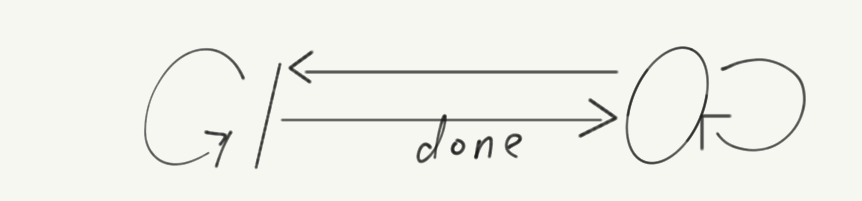
\includegraphics[scale=0.5]{Zzz1.png}
		\caption{The state machine 3.1.3.1}
		\label{fig:1}
	\end{figure}

    $$ 
    \begin{cases}
    E_1=1+\frac{1}{2}E_1+\frac{1}{2} \times 0 \\
    E_2=1+\frac{1}{2}E_2+\frac{1}{2}E_1 
    \end{cases}
    $$
    
    $$
    \Rightarrow \begin{cases}
    E_1=2\\
    E_2=4\\
    \end{cases}
    $$
    $$
\Rightarrow E[T_{10}]=1+\frac{1}{2}E_1+\frac{1}{2}E_2=4
    $$

    \begin{figure}[H]
		\centering
		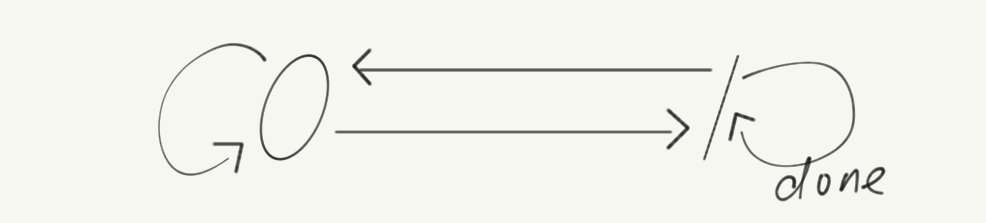
\includegraphics[scale=0.5]{Zzz2.png}
		\caption{The state machine 3.1.3.2}
		\label{fig:1}
	\end{figure}
    $$
    \begin{cases}
    E_1=1+\frac{1}{2}E_1+\frac{1}{2}E_2\\
    E_2=1+\frac{1}{2}E_1+\frac{1}{2} \times 0
    \end{cases}
    $$

    $$
    \Rightarrow \begin{cases}
    E_1=6\\
    E_2=4\\
    \end{cases}
    $$
    $$
\Rightarrow E[T_{11}]=1+\frac{1}{2}E_1+\frac{1}{2}E_2=6
    $$
    
    
	



	\textbf{Exercise 3.2}\par
	There are 2 states of the coin, which are 0 and 1. Assuming the probability of the event under each state is $P_1$ and $P_2$ respectively, we have
	$$
	\Rightarrow \begin{cases}
	P_1=\frac{1}{2}P_1+\frac{1}{2}P_2\\
	P_2=\frac{1}{2}\times 0+\frac{1}{2}\times 1\\
	\end{cases}
	$$
	$$\Rightarrow
	\begin{cases}
	P_1=\frac{1}{2}\\
	P_2=\frac{1}{2}\\
	\end{cases}
	$$
	$$
	\Rightarrow Pr[\varepsilon]=\frac{1}{2}(P_1+P_2)=\frac{1}{2}
	$$







	
	



	
	\textbf{Exercise 3.3}\par
	
	\textbf{ 1.}   There are 4 states of last bit pair of $\{x\}$ and $\{y\}$ sequence, which are $\{0,0\},\{1,0\},\{0,1\} and \{1,1\}$. Assuming the expectation of $T$ under each state is $E_1,E_2,E_3,E_4$ respectively, we have
    $$
        \begin{cases}
        E_1=1+\frac{1}{4}E_1+\frac{1}{4}E_2+\frac{1}{4}E_3+\frac{1}{4}E_4\\
        E_2=1+\frac{1}{4}E_2+\frac{1}{4}E_4\\
        E_3=1+\frac{1}{4}E_1+\frac{1}{4}E_2\\
        E_4=1+\frac{1}{4}E_2\\
        \end{cases}
    $$
   $$
   	\Rightarrow 
	\begin{cases}
	E_1=\frac{384}{121}\\
	E_2=\frac{272}{121}\\
	E_3=\frac{20}{11}\\
	E_4=\frac{16}{11}
	\end{cases}
	$$
	$$\Rightarrow E[T]=\frac{1}{4}(E_1+E_2+E_3+E_4) = \frac{384}{121} $$\par
	\textbf{ 2.}
	
	\textbf{(a)}   Similar to the solution above, assuming the prabability of the event "10 appears in x before 11 appears in y" under each state is $Pra_1,Pra_2,Pra_3,Pra_4$, we have
	
	\begin{figure}[H]
		\centering
		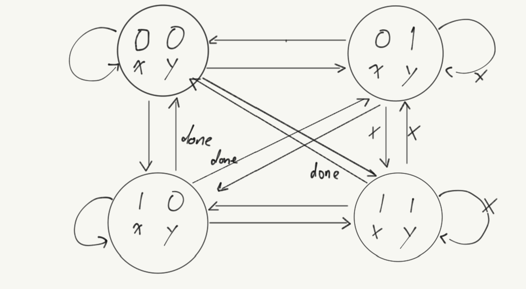
\includegraphics[scale=0.9]{Zzz.png}
		\caption{The state machine 3.3.2}
		\label{fig:3}
	\end{figure}


	$$
	\begin{cases}
	Pra_1=\frac{1}{4}Pra_1+\frac{1}{4}Pra_2+\frac{1}{4}Pra_3+\frac{1}{4}Pra_4\\
	Pra_2=\frac{1}{2}+\frac{1}{4}Pra_2+\frac{1}{4}Pra_4\\
	Pra_3=\frac{1}{4}Pra_1+\frac{1}{4}Pra_2\\
	Pra_4=\frac{1}{4}+\frac{1}{4}Pra_2\\
	\end{cases}
	$$
    $$
	\Rightarrow 
	\begin{cases}
	Pra_1=\frac{65}{121}\\
	Pra_2=\frac{9}{11}\\
	Pra_3=\frac{41}{121}\\
	Pra_4=\frac{5}{11}
	\end{cases}
	$$
	
	$$\Rightarrow Pra=\frac{1}{4}(Pra_1+Pra_2+Pra_3+Pra_4) = \frac{65}{121} $$\\
	
	\textbf{(b)}   Similar to the solution above, assuming the prabability of the event "10 appears in x at the same time with 11 appears in y" under each state is $Prb_1,Prb_2,Prb_3,Prb_4$, we have
	$$
	\begin{cases}
	Prb_1=\frac{1}{4}Prb_1+\frac{1}{4}Prb_2+\frac{1}{4}Prb_3+\frac{1}{4}Prb_4\\
	Prb_2=\frac{1}{4}Prb_2+\frac{1}{4}Prb_4\\
	Prb_3=\frac{1}{4}Prb_1+\frac{1}{4}Prb_2\\
	Prb_4=\frac{1}{4}+\frac{1}{4}Prb_2\\
	\end{cases}
	$$
	$$
	\Rightarrow 
	\begin{cases}
	Prb_1=\frac{17}{121}\\
	Prb_2=\frac{1}{11}\\
	Prb_3=\frac{7}{121}\\
	Prb_4=\frac{3}{11}
	\end{cases}
	$$
	
	$$\Rightarrow Prb=\frac{1}{4}(Prb_1+Prb_2+Prb_3+Prb_4) = \frac{17}{121} $$\\
	
	\textbf{(c)}   Similar to the solution above, assuming the prabability of the event "10 appears in x after 11 appears in y" under each state is $Prc_1,Prc_2,Prc_3,Prc_4$, we have
	$$
	\begin{cases}
	Prc_1=\frac{1}{4}Prc_1+\frac{1}{4}Prc_2+\frac{1}{4}Prc_3+\frac{1}{4}Prc_4\\
	Prc_2=\frac{1}{4}Pra_2+\frac{1}{4}Pra_4\\
	Prc_3=\frac{1}{2}+\frac{1}{4}Prc_1+\frac{1}{4}Prc_2\\
	Prc_4=\frac{1}{4}+\frac{1}{4}Prc_2\\
	\end{cases}
	$$
	$$	\Rightarrow 
	\begin{cases}
	Prc_1=\frac{39}{121}\\
	Prc_2=\frac{1}{11}\\
	Prc_3=\frac{73}{121}\\
	Prc_4=\frac{3}{11}
	\end{cases}
	$$


	$$\Rightarrow Prc=\frac{1}{4}(Prc_1+Prc_2+Prc_3+Prc_4) = \frac{39}{121} $$\\
	





	\textbf{Exercise 3.4}\par

	\textbf{1.}\par We have $Pr(T=n)=p(1-p)^{n-1}$,$n=1,2,\cdots$ Thus, $T$ obeys geometric distribution.\par
	Then $$E(T^2)=\sum_{n=1}^\infty n^2p(1-p)^{n-1}$$.\par
	Here, we have 
	$$
	\sum_{n=1}^\infty nx^{n-1}=(\sum_{n=1}^\infty x^n)'=(\frac{x}{1-x})'=\frac{1}{(1-x)^2}
	$$
	and 
	$$
	\sum_{n=1}^\infty n^2x^{n-1}=(\sum_{n=1}^\infty nx^n)'=(x\sum_{n=1}^\infty nx^{n-1})'=(\frac{x}{(1-x)^2})'=\frac{1+x}{(1-x)^3}
	$$
	Then we order $x=1-p$. We have 
	$$
	E(T^2)=\sum_{n=1}^\infty n^2p(1-p)^{n-1}=p\sum_{n=1}^\infty n^2(1-p)^{n-1}=p\times \frac{2-p}{p^3}=\frac{2-p}{p^2}
	$$
	\textbf{2.}\par
	\begin{align*}
	E(\frac{1}{T})&=\sum_{n=1}^\infty \frac{1}{n} p(1-p)^{n-1}\\
	&=\frac{p}{1-p}\sum_{n=1}^\infty \frac{(1-p)^n}{n}\\
	&=\frac{p}{1-p}\sum_{n=1}^\infty \int_{1}^{p}-(1-p)^{n-1}\,dp\\
	&=\frac{p}{1-p}\int_{1}^{p}\{\sum_{n=1}^\infty -(1-p)^{n-1}\}\,dp\\
	&=\frac{p}{1-p}\int_{1}^{p}-\lim_{n\to\infty}\frac{1-(1-p)^{n}}{p}\,dp\\
	&=\frac{p}{1-p}\int_{1}^{p}-\frac{1}{p}\,dp\\
	&=-\frac{p\ln p}{1-p}
	\end{align*}\par


	\textbf{Question}\par


	\textbf{1.}   In Exercise 3.3 of Homework 3, we are required to solve  E[T], where $T := min(T_{10} (x),T_{11} (y)).$ We use transformation equation of state to solve the problem. However, if we change this question to $T := max(T_{10} (x),T_{11} (y))$, it is rather difficult to set up transformation equation because we do not know whether 10 has existed in X or 11 has existed in Y, or neither has happened. So we want to know how to solve the problem if $T := max(T_{10} (x),T_{11} (y))$.\par
	\textbf{2.}   Consider that in one infinite sequence the same as Exercise 3.2, we let $T:=T_{11}-T_{10}$. It means the number of bits from the first appearance of 10 to the first appearance of 11. How can we calculate E[T]? 

	
\end{document}

